\chapter{State of research}
In this chapter we will see some examples of tables and figures.

\section{Fabrication of AlScN based Contour Mode resonators}
After the results achieved by Lozzi \cite{lozzi_al083sc017n_2019} with 17.5\% Sc AlScN the objective has shifted to optimie fabrication 
\subsection{Sputtering deposition optimisaton}
Carried over from the doctoral studies of Kaitlin M. Howell \cite{howell_dielectric_2019} the first objective of research in AlScN technologies is to optimize the deposition of AlScN in the Spider600 cluster tool at CMi. The Spider600 is a sputtering cluster which allows deposition from different targets in the same fabrication round, without breaking the vacuum between layers. This tools allows or a reactive sputtering of full stacks of the resonator structure. To optimize the deposition three main results were kept in consideration: density of abnormal oriented grains on an SEM image, Rocking curve of X-ray diffraction and measured coupling coefficient $k_t^2$ to gain as much insight as possible on the process. 

\subsection{Effect of gas flows}
it is possible to set two gas flows in the Spider600, Argon as the sputtering gas for the target and Nitrogen as the reactive gas that will form the AlScN film. Three different combination of gas flows were tested: 0/50 10/40 20/30 (Ar gas flux in sccm / \ch{N2} gas flux in sccm). Analysis at the SEM shows that an increase of argon results in a lower density of AOG (see Figure \ref{fig:AOG}). SEM does not tell the whole story though, as XRD is used to characterize the crystal orientation of the film. It is shown from XRD that the rocking curve 

\begin{figure}[ht]
	\begin{subfigure}{.33\textwidth}
		\centering
		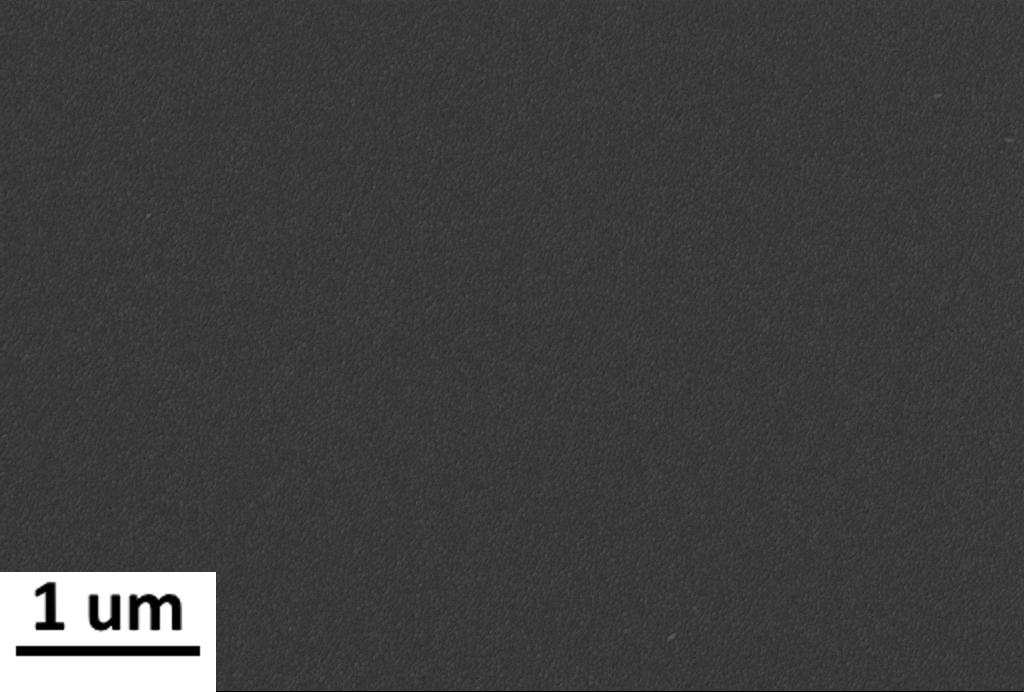
\includegraphics[width=.9\linewidth]{images/SEM/88344_middle_01}
		\caption{20/30}
	\end{subfigure}
	\begin{subfigure}{.33\textwidth}
		\centering
		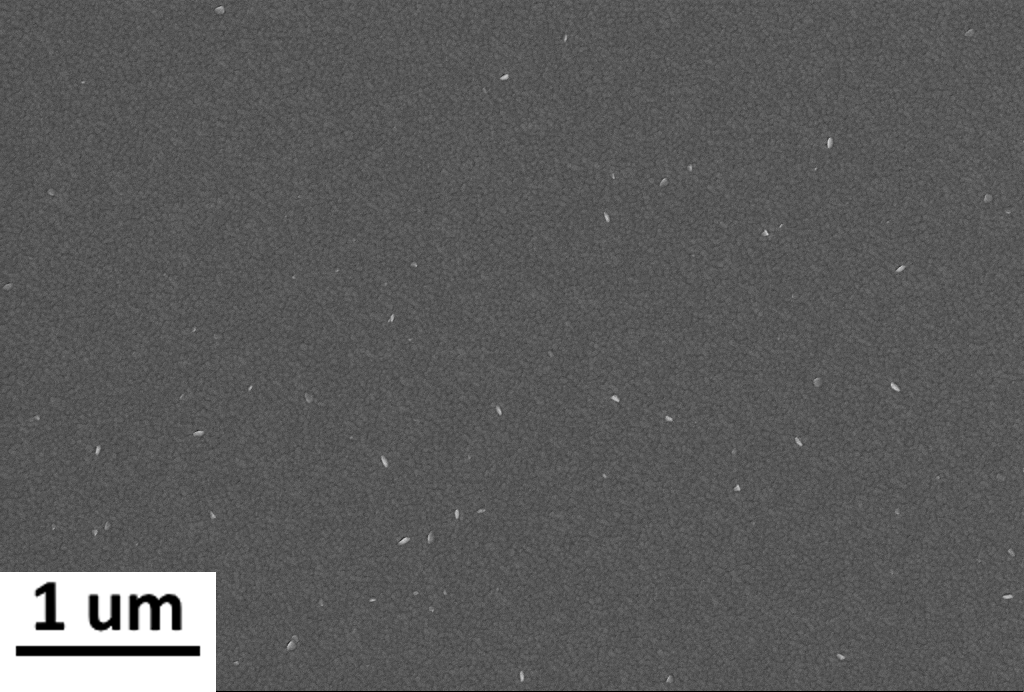
\includegraphics[width=.9\linewidth]{images/SEM/88384_middle_01}
		\caption{10/40}
	\end{subfigure}
\begin{subfigure}{.33\textwidth}
	\centering
	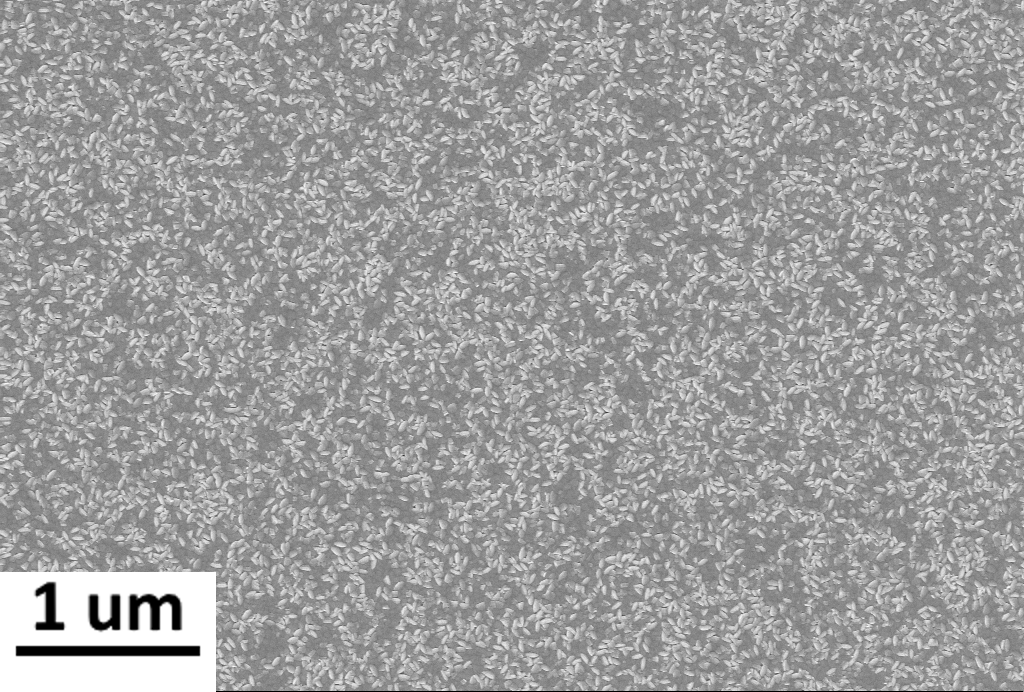
\includegraphics[width=.9\linewidth]{images/SEM/88387_middle_01}
	\caption{0/50}
\end{subfigure}
\caption{Abnormally oriented grains as function of gas flow rates (sccm \ch{Ar} / sccm \ch{N2} )}
\label{fig:AOG}
\end{figure}
	
\subsection{Effect of biasing power in high-resistive wafers}
\label{ssec:HR}
In multiple occasion, both with \ch{Al_{0.6}Sc_{0.4}N} and with \ch{Al_{0.83}Sc_{0.17}N} it was noticed that according to the substrate of the deposition the $k_t^2$ was affected. Under the same fabrication process, High resistive (HR) wafers showed a systematic lower coupling compared to standard Test wafers. The Test wafers are SSP 100mm <100> with resistivity of  max 100 $\Omega cm$. HR wafers are DSP 100mm <100> with resistivity higher than 10k $\Omega cm$. According to \cite{sandu_impact_2020} an increase of RF bias power in deposition will lead to a random growth of crystal. it was our belief that in the case of HR wafers the extra resistance of the wafer has to be offset by increasing the bias power, on a range of 3, 4, 6 and 8 W. After XRD analysis it is shown that the theta2theta peak at 36° (Corresponding to (0002) AlScN) has the maximum count intensity at 4W compared to the 2W of the paper, while according to the previous results the crystalline peak disappears with powers higher than 6W. On the side of rocking curve the broadening of the FWHM is proportional to the power. According to this first measurement the growth on an HR wafer benefits from a bias increase but there is a tradeoff between the crystallinity of the film (given from the theta2theta) and the ordered vertical growth of it (given by the Rocking Curve). Investigation is ongoing to find the soft point.

\subsection{Effects of bottom electrode coverage}
\label{ssec:bottom}
According to literature \cite{howell_effect_2019} \cite{xiong_influence_2010} the best condition for the growth of an AlN film is to have a seed layer of Pt, that will act also as a bottom electrode to actuate the device. Since adhesion of Pt to the substrate is extremely low, an adhesion layer of Ti is usually employed to solve the problem. The best possible condition for crystal growth happens when the whole wafer is coated with Pt, but this is detrimental for the device performances, because this very large bottom electrode will introduce enormous parasitic capacitances that will reduced the electrical $k_t^2$. in previous iterations of the project the bottom electrode was patterned with Lift-off so that the Pt electrode would be only below the main resonator body. This meant that while the more "important" regions of the wafers were grown over a Pt substrate, the vas majority of the \ch{AlScN} was grown on bare Si. To run these tests the same deposition was done over a full bottom and a patterned bottom and analyzed under XRD.  


\begin{figure}
	\begin{subfigure}{.5\textwidth}
		\centering
		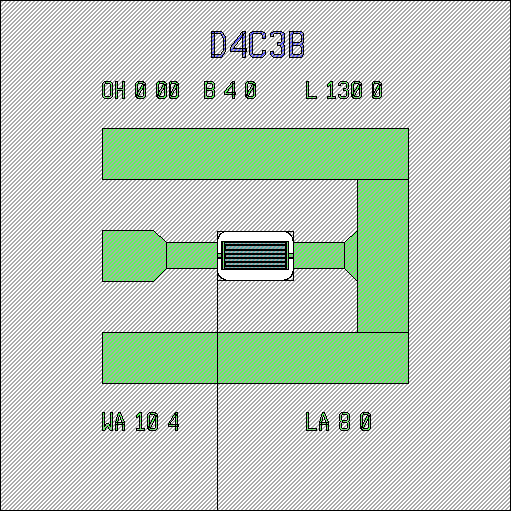
\includegraphics[width=0.8\linewidth]{images/Coverage/low}
		\caption{Low coverage}
		\label{subfig:low}
	\end{subfigure}
	\begin{subfigure}{.5\textwidth}
		\centering
		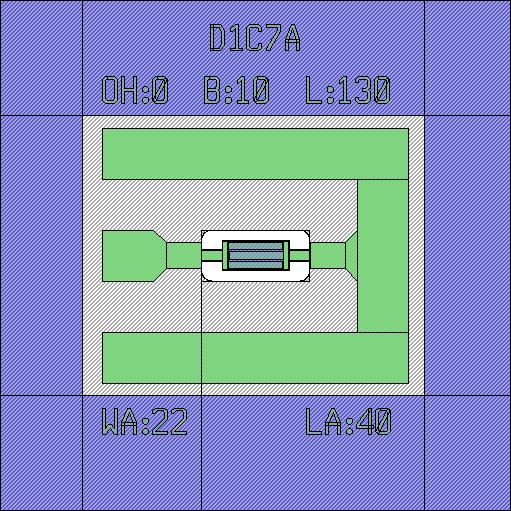
\includegraphics[width=0.8\linewidth]{images/Coverage/high}
		\caption{High coverage}
		\label{subfig:high}
	\end{subfigure}
	\caption{Different coverage approaches to design of resonator. Parasitics rise when the top metal (green) overlaps with the bottom (blue)}
\end{figure}

\subsection{AlScN on AlN}
In the strive to achieve a better cristallinity for \ch{Al_{0.6}Sc_{0.4}N} another choice was to follow the approach proposed in \cite{parsapour_ex-situ_2017} for \ch{Al_{0.83}Sc_{0.17}N}. The underlining idea is that the crystalline growth of AlScN can be promoted by a thin film of AlN above the bottom Pt electrode. A batch of 6 wafers was prepared, 2 test wafers and 4 HR wafers, at different Bias power with patterned and non-patterned bottom electrode. Coherently to the result shown in \ref{ssec:HR} XRD measurements show that on both Test Wafers and HR wafers, at the same power level and substrate type, the rocking curve peak is narrower for the AlScN wafers where a growth promotion layer of AlN was put. Interesting, the theta2theta peak is higher in AlN-buffered AlScN only in the wafers with the lowest power. In wafers with the higher bias power the AlN-buffered depostions have a lower theta2theta peak compared to the ones directly deposited on the bottom Pt electrode. The main interest in this technique is not only related to the improvement of film quality over Si substrates, but can help in case of non crystalline substrates, as in the case of \cite{parsapour_ex-situ_2017} where AlScN was deposited over a \ch{SiO2} layer.
The analysis described in Subsection \ref{ssec:HR} showed that for both HR and test wafers, the usage of a patterned bottom electrode with high coverage sligthly increases the rocking curve (between 5 and 10 \%) 

\subsection{Inductively coupled plasma etching}

\section{CMR based oscillator}

\section{Published Papers}
\begin{itemize}
	\item A.Lozzi, M. Liffredo \textit{et als} "Evidence of Smaller 1/F Noise in AlScN-Based Oscillators Compared to AlN-Based Oscillators" \cite{lozzi_evidence_2020}
\end{itemize}
\section{Attended Courses}
\begin{itemize}
	\item Scanning electron microscopy techniques
	\item Techniques for handling noise and variability in analog circuits
	\item Energy efficient autonomous wireless devices
	\item Design of Experiments
	\item Enterpreneurial Opportunities Identification and Exploitation
	\item Piezoelectric Materials Properties and Devices
\end{itemize}